%\appendix

\subsection{Analysis of Independent Thompson Sampling: Proof of Theorem~\ref{thm:TS}} \label{proof:TS}

Fix a sub-optimal arm $k$. Several cases need to be considered depending on the relative position of $p_k$ and $p_{k^*}$ with respect to the threshold. All cases can be treated similarly and to fix the ideas, we consider the case $p_{k^*} \geq \theta > p_k$, which is illustrated below. In that case $d^*_k = 2\theta - p_{k^*}$ satisfies $p_k \leq d_{k}^* \leq \theta$.

\begin{figure}[h]\centering
 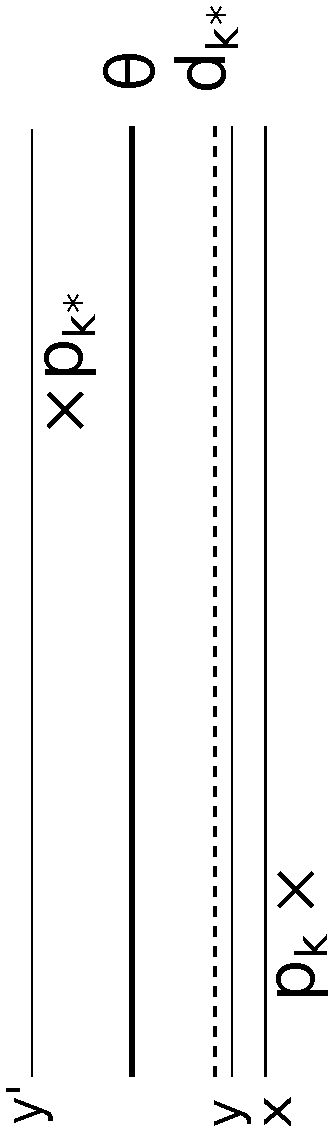
\includegraphics[height=7cm,angle=-90]{dosefinding/illustration}
\end{figure}

Let $x,y \in ]0,1[^2$ be such that $p_k < x < y < d_{k^*}$, that will be chosen later. Define $y' = 2\theta - y > \theta$ the symmetric of $y$ with respect to the threshold (see the above illustration). We denote by  $\hat{\mu}_k(t)$ the empirical mean of the toxicity responses gathered from dose $k$ up to the end of round $t$ and recall $\theta_k(t)$ is the sample from the Beta posterior on $p_k$ after $t$ rounds that is used in the Thompson Sampling algorithm. Inspired by the analysis of \cite{AGAISTAT13}, we introduce the following two events, that are quite likely to happen when enough samples of arm $k$ have been gathered: 
\begin{eqnarray*}
 E_k^\mu (t) & = & \left(\hat{\mu}_k(t) \leq x\right) \ \ \ \text{and} \ \ \ E_k^\theta (t)  =  \left({\theta}_k(t) \leq y\right).
\end{eqnarray*}

The expected number of allocations of dose $k$ is then decomposed in the following way 
\begin{align*}
 \bE[N_k(T)] = &\underbrace{\sum_{t=0}^{T-1}\bP\left(D_{t+1} = k, E_k^\mu(t),E_k^\theta(t)\right)}_{(I)}+ \underbrace{\sum_{t=0}^{T-1}\bP\left(D_{t+1} = k, E_k^\mu(t),\overline{E_k^\theta(t)}\right)}_{(II)}
 \\ &
 	+ \underbrace{\sum_{t=0}^{T-1}\bP\left(D_{t+1} = k, \overline{E_k^\mu(t)}\right)}_{(III)}  
\end{align*}
Terms (II) and (III) are easily controlled using some concentration inequalities and the so-called Beta-Binomial trick, that is the fact that the CDF of a Beta distribution with parameters $a$ and $b$, $F^{\text{Beta}}_{a,b}$, is related to the CDF of a binomial distribution with parameter $n,x$, $F^{B}_{n,x}$, in the following way: \[F^{\text{Beta}}_{a,b}(x) = 1 - F^{B}_{a+b-1, x}(a - 1).\] Term (III) is very small as arm $k$ is unlikely to be drawn often while its empirical mean falls above $x > p_k$ and term (II) grows logarithmically with $T$. More precisely, it can be shown using Lemma 3 and 4 in \cite{AGAISTAT13} that 
\[
 (II)  \leq  \frac{\log(T)}{d(x,y)} + 1 \ \ \ \text{ and } \ \ \ (III)  \leq  \frac{1}{d(x,y)} + 1.
\] 
The tricky part of the analysis is to control term (I), that is to upper bound the number of selections of dose $k$ when both the empirical mean and the Thompson sample for dose $k$ fall close to the true mean $p_k$. For this purpose, one can prove a counterpart of Lemma 1 in \cite{AGAISTAT13} that relates the probability of selecting dose $k$ to that of selecting the MTD $k^*$. 

\begin{lemma}\label{lem:CrucialAG}Define $p_{y}(t) : = \bP\left({\theta}_{k^*}(t) \in [y,y'] | \cF_{t}\right)$, where $\cF_{s}$ is the filtration generated by the observation up to the end of round $s$. Then 
\begin{align*}
&\bP\left(D_{t+1} = k | E_{k}^\theta(t+1),\cF_{t}\right)\leq \frac{1-p_{y}(t)}{p_y(t)}\bP\left(D_{t+1} = k^* | E_k^\theta(t+1),\cF_{t}\right).
\end{align*}
\end{lemma}

\begin{proof} The proof is inspired of that of Lemma 1 in \cite{AGAISTAT13}. We introduce the event in which the Thompson sample for dose $k$ is the closest to the threshold $\theta$ among all sub-optimal doses:
\[M_k(t) = \{ |\theta - \theta_k(t)| \geq |\theta - \theta_\ell(t)| \forall \ell \neq k^*\}.\]
On the one hand, one has
\begin{align*}
 \bP\left(D_{t+1} = k^* | E_k^\theta(t+1),\cF_t\right)& \geq
 	\bP\left(D_{t+1} = k^*,M_k(t) | E_k^\theta(t+1),\cF_t\right)
 \\ & \geq
   \bP\left(\theta_{k^*}(t) \in [y,y'],M_k(t) | E_k^\theta(t+1),\cF_t\right) 
\\ & =
	p_y(t) \times \bP\left(M_k(t) | E_k^\theta(t+1),\cF_t\right).
\end{align*}
On the other hand, it holds that 
\begin{align*} \bP\left(D_{t+1} = k | E_k^\theta(t+1),\cF_t\right)
 & \leq \bP\left(\theta_{k^*}(t) \notin [y, y'], M_k(t) | E_k^\theta(t+1),\cF_t\right)
\\ & = (1 - p_y(t)) \times \bP\left(M_k(t) | E_k^\theta(t+1),\cF_t\right).
\end{align*}
Combining the two inequalities yields Lemma~\ref{lem:CrucialAG}.
\end{proof}

Using the same steps as \cite{AGAISTAT13} yields an upper bound on the first term:
\[(I) \leq \sum_{j=1}^{T-1}\bE\left[\frac{1}{p_y(\tau_{j})} - 1\right],\]
where $\tau_j$ is the time instant at which dose $k$ is selected for the $j$-th time. The expectation of $1/p_y(\tau_{j})$ can be explicitly written 
\[\bE\left[\frac{1}{p_y(\tau_{j})}\right] =\sum_{s=0}^j \frac{f^B_{j,p_{k^*}}(s)}{\bP\left(y \leq X_{s+1,j-s+1} \leq y'\right)} \]
where $f^B_{n,x}$ stands for the pdf of a Binomial distribution and $X_{a,b}$ denotes a random variable that has a $\mathrm{Beta}(a,b)$ distribution. The following lemma is crucial to finish the proof. This original result was specifically obtained for the MTD identification problem and is needed to control the probability that a Beta distributed random variable fall inside an interval, that is $\bP\left(y \leq X_{s+1,j-s+1} \leq y'\right)$.


\begin{lemma}\label{lem:Technical} There exists $j_0$ such that, for all $j \geq j_0$,
\begin{align*}
&\forall s \in \{0,\dots, j\}, \ \ \bP\left(y \leq X_{s+1,j-s+1} \leq y'\right) \geq \frac{1}{2}\min  \left\{\bP\left(X_{s+1,j+s+1} \geq y\right) ; \bP\left(X_{s+1,j+s+1} \leq y'\right)\right\}
\end{align*}
\end{lemma}

Using Lemma~\ref{lem:Technical} and the Beta-Binomial trick, one can write, for $j \geq j_0$, 
\begin{align}
\nonumber
\bE\left[\frac{1}{p_y(\tau_{j})}\right]
 & \leq
\sum_{s=0}^j \frac{2f^B_{j,p_{k^*}}(s)}{\bP\left(X_{s+1,j+s+1} \geq y\right)}+\sum_{s=0}^j \frac{2f^B_{j,p_{k^*}}(s)}{\bP\left(X_{s+1,j+s+1} \leq y'\right)} 
 \\ \nonumber & =
 \sum_{s=0}^j \frac{2f^B_{j,p_{k^*}}(s)}{F^B_{j+1,y}(s)} + \sum_{s=0}^j \frac{2f^B_{j,p_{k^*}}(s)}{1-F^B_{j+1,y'}(s)}
 \\ & = \sum_{s=0}^j \frac{2f^B_{j,p_{k^*}}(s)}{F^B_{j+1,y}(s)} + \sum_{s=0}^j \frac{2f^B_{j,1-p_{k^*}}(s)}{F^B_{j+1,1-y'}(s)},\label{eq:star}
\end{align}
where the last equality relies on the following properties of the Binomial distribution \[f^B_{n,x}(s) = f^B_{n,1-x}(n-s) \ \ \text{and} \ \ F^B_{n,x}(s) = 1 - F_{n,1-x}(n-s-1)\]
and a change of variable in the second sum. 

Now the following upper bound can be extracted from the proof of Lemma 3 in \cite{AGAISTAT13}. 

\begin{lemma}\label{lem:UB} Fix $u$ and $v$ such that $u < v$ and let $\Delta = v - u$. Then 
\begin{align*}
\sum_{s=0}^j \frac{f^B_{j,v}(s)}{F^B_{j,u}(s)} \leq
 \left\{\begin{array}{cl}
 1 + \frac{3}{\Delta} & \text{if } j < {8}/\Delta,
 \\
 1 + \Theta\left(e^{-\Delta^2 j /2} + \frac{1}{(j+1)\Delta^2}e^{-2\Delta^2 j} + \frac{1}{e^{\Delta^2j/4} - 1}\right) & \text{else.} 
\end{array}
\right.
\end{align*}
\end{lemma}

Each of the two sums in \eqref{eq:star} can be upper bounded using Lemma~\ref{lem:UB}. Letting $\Delta_1 = p_{k^*} - y$ and $\Delta_2 = y' - p_{k^*}$, one obtains  
\begin{align*}
 (I) \leq &
 	\sum_{j=1}^{j_0} \bE\left[\frac{1}{p_y(\tau_{j})} \right]
 	- j_0 + \frac{24}{\Delta_1^2} + \frac{24}{\Delta_2^2} 
\\ &
	+ C \sum_{j=0}^{T-1} \left[e^{-\Delta_1^2 j /2} + \frac{1}{(j+1)\Delta_1^2}e^{-2\Delta_1^2 j} + \frac{1}{e^{\Delta_1^2j/4} - 1}\right]
\\ &
	+ C \sum_{j=0}^{T-1} \left[e^{-\Delta_2^2 j /2} + \frac{1}{(j+1)\Delta_2^2}e^{-2\Delta_2^2 j} + \frac{1}{e^{\Delta_2^2j/4} - 1}\right], 
\end{align*}
which is a constant (as the series have a finite sum) that only depends on $y, \theta$ and $p_{k^*}$ (through $y'$ and the gaps $\Delta_1$ and $\Delta_2$ defined above). 

Putting things together, we proved that for every $x$ and $y$ satisfying $p_k < x < y < d_{k^*}$, the number of selections of dose $k$ is upper bounded as 
\[ \bE[N_k(T)] \leq \frac{1}{d(x,y)}\log(T) + C_{x,y,\theta,\bm p}\]
for some constant that depends on the toxicity probabilities, the threshold $\theta$ and the choice of $x$ and $y$. Now, picking $x$ and $y$ such that $d(x,y) = \frac{d(p_k,d_{k^*})}{1+\epsilon}$ yield the result. 

\qed 

\paragraph{Proof of Lemma~\ref{lem:Technical}.} The proof uses the two equalities below
\begin{align}
 \bP\left(y \leq X_{s+1,j-s+1} \leq y'\right) & = \bP\left(X_{s+1,j-s+1} \geq y\right) - \bP\left(X_{s+1,j-s+1} \geq y'\right)\label{ForSmallS}
\\ 
\bP\left(y \leq X_{s+1,j-s+1} \leq y'\right)
 & = \bP\left(X_{s+1,j-s+1} \leq y'\right) - \bP\left(X_{s+1,j-s+1} \leq y\right),\label{ForLargeS}
\end{align}
as well as the Sanov inequalities: if $S_{n,x}$ is a binomial distribution with parameters $n$ and $x$, then 
\begin{align}
\nonumber
\frac{e^{-n\kl(k/n,x)}}{n+1}
& \leq \bP\left(S_{n,x} \geq k\right) 
\\ & \leq e^{-n\kl(k/n,x)} \ \ \text{if } \ k > xn \label{Sanov}
\\ \nonumber
\frac{e^{-n\kl(k/n,x)}}{n+1}
& \leq \bP\left(S_{n,x} \leq k\right)
\\ & \leq
	e^{-n\kl(k/n,x)} \ \ \text{if } \ k < xn \label{SanovMin}
\end{align}

We prove the inequality considering 4 cases. We define $\ymid = \frac{y+y'}{2}$. 

\paragraph{Case 1: $\bm{s < (j+1)y}$} Starting from equality \eqref{ForSmallS} and using the Beta-Binomial trick yields  
\begin{align*}
&\bP\left(y \leq X_{s+1,j-s+1} \leq y'\right) = \bP\left(S_{j+1,y} \leq s\right) - \bP\left(S_{j+1,y'} \leq s\right).
\end{align*}
Using Sanov inequalities, we shall prove that there exists some $j_1$ such that if $j\geq j_1$, 
\[\forall s \leq (j+1)y, \ \ \bP\left(S_{j+1,y'} \leq s\right) \leq \frac{1}{2}\bP\left(S_{j+1,y} \leq s\right).\]
As $s$ is smaller than the mean of the two Binomial distributions, by \eqref{SanovMin} it is sufficient to prove that 
\begin{align*}
&\forall s \leq (j+1)y,
\ \ e^{-(j+1)\kl\left(\frac{s}{j+1} , y'\right)} \leq \frac{1}{2(j+2)}e^{-(j+1)\kl\left(\frac{s}{j+1} , y\right)}
\end{align*}
which in turn is equivalent to 
\begin{align*}
&\forall s \leq (j+1)y,
\ \ \kl\left(\frac{s}{j+1} , y'\right)  -  \kl\left(\frac{s}{j+1} , y\right) \geq \frac{\log(2(j+2))}{j+1}.
\end{align*}
As the function in the left-hand side is non-increasing in $s$, a sufficient condition is that $j$ satisfies 
\[ \kl\left(y , y'\right)\geq \frac{\log(2(j+2))}{j+1},\]
which is the case for $j$ superior to some $j_1$. Thus, for $j\geq j_1$, 
\begin{align*}
\bP\left(y \leq X_{s+1,j-s+1} \leq y'\right)\geq \frac{1}{2}\bP\left(S_{j+1,y} \leq s\right)= \frac{1}{2}\bP\left(X_{s+1,j-s+1} \geq y\right).
\end{align*}

\paragraph{Case 2: $\bm{(j+1)y \leq s \leq (j+1)\ymid}$} Starting from equality \eqref{ForSmallS} and using the Beta-Binomial trick and the upper bound in \eqref{SanovMin} yields 
\begin{align*}
\bP\left(y \leq X_{s+1,j-s+1} \leq y'\right) 
 & \geq \bP\left(S_{j+1,y} \leq s\right) - e^{-(j+1)\kl\left(\frac{s}{j+1} , y'\right)}
\\ & \geq \bP\left(S_{j+1,y} \leq s\right) - e^{-(j+1)\kl\left(\ymid , y'\right)}. 
\end{align*}
The median of $S_{j+1,y}$ is $\lfloor(j+1)y\rfloor$ or $\lceil(j+1)y\rceil$. As $s \leq  (j+1)y$, it holds that $\bP\left(S_{j+1,y} \leq s\right) \geq \frac{1}{2}$. Therefore, for all $j \geq j_2 := \frac{\ln 4}{\kl(\ymid,y')}-1$, 
\[e^{-(j+1)\kl\left(\ymid , y'\right)} \leq \frac{1}{4} \leq \frac{1}{2}\bP\left(S_{j+1,y} \leq s\right).\]
Therefore if $j \geq j_2$, $\bP\left(y \leq X_{s+1,j-s+1} \leq y'\right)  \geq \frac{1}{2}\bP\left(X_{s+1,j-s+1} \geq y\right)$.

\paragraph{Case 3: $\bm{(j+1)\ymid \leq s \leq (j+1)y'}$} Starting from equality \eqref{ForLargeS} and using the Beta-Binomial trick and the upper bound in \eqref{Sanov} yields 
\begin{align*}
 \bP\left(y \leq X_{s+1,j-s+1} \leq y'\right) & \geq \bP\left(S_{j+1,y'} \geq s\right) - e^{-(j+1)\kl\left(\frac{s}{j+1} , y\right)}
\\ & \geq \bP\left(S_{j+1,y'} \geq s\right) - e^{-(j+1)\kl\left(\ymid , y\right)}. 
\end{align*}
The median of $S_{j+1,y'}$ is $\lfloor(j+1)y'\rfloor$ or $\lceil(j+1)y'\rceil$. As $s \leq  (j+1)y'$, it holds that $\bP\left(S_{j+1,y'} \geq s\right) \geq \frac{1}{2}$. Therefore, for all $j \geq j_3 := \frac{\ln 4}{\kl(\ymid,y)}-1$, 
\[e^{-(j+1)\kl\left(\ymid , y\right)} \leq \frac{1}{4} \leq \frac{1}{2}\bP\left(S_{j+1,y'} \geq s\right).\]
Therefore if $j \geq j_3$, $\bP\left(y \leq X_{s+1,j-s+1} \leq y'\right)  \geq \frac{1}{2}\bP\left(X_{s+1,j-s+1} \leq y'\right)$.

\paragraph{Case 4: $\bm{s > (j+1)y'}$} Starting from equality \eqref{ForLargeS} and using the Beta-Binomial trick yields  
\[\bP\left(y \leq X_{s+1,j-s+1} \leq y'\right)  =  \bP\left(S_{j+1,y'} \geq s\right) - \bP\left(S_{j+1,y} \geq s\right).\]
Using Sanov inequalities, we shall prove that there exists some $j_4$ such that if $j\geq j_4$, 
\[\forall s \geq (j+1)y', \ \ \bP\left(S_{j+1,y} \geq s\right) \leq \frac{1}{2}\bP\left(S_{j+1,y'} \geq s\right).\]
As $s$ is larger than the mean of the two Binomial distributions, by \eqref{Sanov} it is sufficient to prove that 
\[\forall s \geq (j+1)y', \ \ e^{-(j+1)\kl\left(\frac{s}{j+1} , y\right)} \leq \frac{1}{2(j+2)}e^{-(j+1)\kl\left(\frac{s}{j+1} , y'\right)}\]
which in turn is equivalent to 
\[\forall s \geq (j+1)y', \ \ \kl\left(\frac{s}{j+1} , y\right)  -  \kl\left(\frac{s}{j+1} , y'\right) \geq \frac{\log(2(j+2))}{j+1}.\]
As the function in the left-hand side is non-decreasing in $s$, a sufficient condition is that $j$ satisfies 
\[ \kl\left(y' , y\right)\geq \frac{\log(2(j+2))}{j+1},\]
which is the case for $j$ superior to some $j_4$. Thus, for $j\geq j_4$, 
\begin{align*}
\bP\left(y \leq X_{s+1,j-s+1} \leq y'\right) 
&\geq \frac{1}{2}\bP\left(S_{j+1,y'} \geq s\right) 
\\ &= \frac{1}{2}\bP\left(X_{s+1,j-s+1} \leq y'\right).
\end{align*}

\paragraph{Conclusion} Letting $j_0 = \max(j_1,j_2,j_3,j_4)$, for all $j\geq j_0$, for every $s \in \{0,\dots,j\}$,
\begin{align*}
&\bP\left(y \leq X_{s+1,j-s+1} \leq y'\right) \geq \frac{1}{2}\min \left\{\bP\left(X_{s+1,j+s+1} \geq y\right) ; \bP\left(X_{s+1,j+s+1} \leq y'\right)\right\}
\end{align*}

\qed


\subsection{Analysis of Sequential Halving: Proof of Theorem~\ref{thm:SH}}
\label{sec:SHproof}

Recall $\hat{d}_k^r = |\theta - \hat{p}_k^t|$ is the empirical distance from the toxicity of dose $k$ to the threshold, where $\hat{p}_k^r$ is the empirical average of the toxicity responses observed for dose $k$ during phase $r$ (based on $t_r$ samples). The central element of the proof is Lemma~\ref{lemma-inversion} below, that controls the probability that dose $k$ seems to be be closer to the threshold than the MTD $k^*$ in phase $r$. Its proof is more sophisticated than that of Lemma 4.2 in \cite{icml2013_karnin13} as several cases need to be considered. 
%
% LEMMA: lemma-inversion
%
\begin{lemma}
\label{lemma-inversion}
Assume that the arm closest to $\theta$ was not eliminated
prior to round $r$.
Then for any arm $k \in S_r$,
\begin{equation}\bP(\hat{d}^r_{k^*} > \hat{d}^r_k) \leq 3 \exp\left(- \frac{t_r}{2}\Delta_k^2\right).\label{toproofin4case}\end{equation}
\end{lemma}
%
% LEMMA PROOF
%
\begin{proof}
For the means $p_{k^*}$ and $p_k$ let $\hat{p}^r_{k^*}$ and $\hat{p}^r_k$ denote their
expected rewards in round $r$, respectively.
We will first derive a probability bound which does not depend on the
ordering of $p_k$ and $p_{k^*}$ w.r.t. $\theta$, and then we will do a case
analysis of the possible orderings to produce our final bound.

The error event can be decomposed as follows. 
\begin{align*}
&\Set{\hat{d}^r_{k^*} > \hat{d}^r_k} =
\\
	&~~~\left( \Set{\hat{p}_{{k^*},r} > \theta}
		\cap \Set{\hat{p}_{k,r} > \theta}
		\cap \Set{\hat{p}_{{k^*},r} - \theta > \hat{p}_{k,r} - \theta}
		\right) \\
	&\cup \left(
		\Set{\hat{p}_{{k^*},r} \le \theta}
		\cap \Set{\hat{p}_{k,r} > \theta}
		\cap \Set{\theta - \hat{p}_{{k^*},r} > \hat{p}_{k,r} - \theta}
		\right) \\
	&\cup \left(
		\Set{\hat{p}_{{k^*},r} > \theta}
		\cap \Set{\hat{p}_{k,r} \le \theta}
		\cap \Set{\hat{p}_{{k^*},r} - \theta > \theta - \hat{p}_{k,r}}
		\right) \\
	&\cup \left(
		\Set{\hat{p}_{{k^*},r} \le \theta}
		\cap \Set{\hat{p}_{k,r} \le \theta}
		\cap \Set{\theta - \hat{p}_{{k^*},r} > \theta - \hat{p}_{k,r}}
		\right)
\end{align*}
From there, we distinguish two cases, in which we show the error event is included in a reunion of events whose probability can be controlled using the Hoeffding's inequality. 

\paragraph{Case 1: $\bm{p_k \geq \theta}$.} In that case, it is very unlikely that $\{\hat{p}_{k,r} < \theta\}$. Hence, we can isolate that event and use the previous decomposition to write
\begin{align*}
&\Set{\hat{d}^r_{k^*} > \hat{d}^r_k} \subseteq 
\\
&\Set{\hat{p}_{k,r} \le \theta} \cup \Set{\hat{p}_{{k^*},r} - \hat{p}_{k,r} > 0}
		\cup \Set{\hat{p}_{k,r} + \hat{p}_{{k^*},r} < 2\theta}
		.
\end{align*}
When $p_k \geq \theta$, irrespective of the position of $p_{k^*}$ with respect to $\theta$, one can justify that $p_k > \theta$, $p_{k^*} - p_{k} < 0$ and ${p}_{k} + {p}_{{k^*}} > 2\theta$ (as $p_k \geq \max(p_{k^*},2\theta - p_{k^*})$ because $k$ is a suboptimal arm larger than the threshold). Therefore, the above three events are unlikely. More precisely, using Hoeffding's inequality yields  
\begin{align*}
\bP(\hat{d}^r_{k^*} > \hat{d}^r_k) 
 &\leq 
	\bP(\hat{p}_{k,r} \le \theta)
	+ \bP(\hat{p}_{{k^*},r} - \hat{p}_{k,r} > 0)
	+ \bP(\hat{p}_{k^*,r} + p_{k,r} < 2\theta)
\\ &\leq 
	\exp\left( -2t_r (\theta - p_k)^2 \right\}
	+ \exp\left\{ - \frac{t_r}{2} (p_{k^*} - p_k)^2 \right\}
\\
	& \hspace{0.4cm} + \exp\left\{ - \frac{t_r}{2} (p_{k^*} + p_k - 2\theta )^2 \right)
\\ &\leq 
	3 \exp\left( -\frac{t_r}{2} \min\left\{(p_{k} - \theta)^2,
		(p_{k} - p_{k^*})^2,
		(p_{k^*}+ p_k - 2\theta)^2
	  \right\} \right)
\\ & = 
	3 \exp\left( -\frac{t_r}{2} \min\left\{
		(p_{k} - p_{k^*})^2,
		(p_{k} - (2\theta - p_{k^*}))^2
	  \right\} \right)
\end{align*}
Equation~\eqref{toproofin4case} follows as $\Delta_k^2 = \min\left\{
		(p_{k} - p_{k^*})^2,
		(p_{k} - (2\theta - p_{k^*}))^2
	  \right\}$. 

\paragraph{Case 2: $\bm{p_k \leq \theta}$.} In that case, the unlikely event is $\{\hat{p}_{k,r} > \theta\}$ and we write 
\begin{align*}
&\Set{\hat{d}^r_{k^*} > \hat{d}^r_k} \subseteq 
\Set{\hat{p}_{k,r} > \theta} \cup \Set{\hat{p}_{{k},r} - \hat{p}_{k^*,r} > 0}\cup \Set{\hat{p}_{k,r} + \hat{p}_{{k^*},r} > 2\theta}.
\end{align*}
When $p_k < \theta$, irrespective of the position of $p_{k^*}$ with respect to $\theta$, one can justify that $p_k < \theta$, $p_{k} - p_{k^*} < 0$ and ${p}_{k} + {p}_{{k^*}} < 2\theta$ (using the fact that $p_k \leq \min(p_{k^*},2\theta - p_{k^*})$). Then from Hoeffding's inequality,  
\begin{align*}
\bP(\hat{d}^r_{k^*} > \hat{d}^r_k) & \leq 
	\bP(\hat{p}_{k,r} > \theta)
	+ \bP(\hat{p}_{{k},r} - \hat{p}_{k^*,r} > 0)
	+ \bP(\hat{p}_{k^*,r} + p_{k,r} > 2\theta)
\\ & \leq 
	\exp\left( -2t_r (\theta - p_k)^2 \right\}
	+ \exp\left\{ - \frac{t_r}{2} (p_{k^*} - p_k)^2 \right\}
\\ & \hspace{0.4cm}
	+ \exp\left\{ - \frac{t_r}{2} (2\theta - p_{k^*} - p_k)^2 \right)
\\ & \leq 
	3 \exp\left( -\frac{t_r}{2} \min\left\{(\theta - p_k)^2,
		(p_{k^*} - p_k)^2,
		(2\theta - p_{k^*} -p_k)^2
	  \right\} \right)
\\ & = 
	3 \exp\left( -\frac{t_r}{2} \min\left\{
		(p_{k^*} - p_{k})^2,
		((2\theta - p_{k^*}) - p_k)^2
	  \right\} \right)
\end{align*}
which proves Equation~\ref{toproofin4case} as $\Delta_k^2 =\min\left\{
		(p_{k^*} - p_{k})^2,
		((2\theta - p_{k^*}) - p_k)^2
	  \right\}$. 
\end{proof}


Building on Lemma~\ref{lemma-inversion}, the next step is to control the probability that the MTD is eliminated in phase $r$. The proof bears strong similarities with that of Lemma~4.3 in \cite{icml2013_karnin13}. It is given below for the sake of completeness. 

%
% LEMMA: lemma-best-survives
%
\begin{lemma}
\label{lemma-best-survives}
The probability that the MTD is eliminated at the end of phase $r$ is at most
\begin{align*}
9 \exp\left(
	- \frac{n}{8 \log_2 K} \cdot \frac{\Delta^2_{k_r}}{k_r}
\right)	
\end{align*}
where $k_r = K/2^{r + 2}$.
\end{lemma}
%
% LEMMA PROOF
%

%
% THEOREM: correctness probability
%
The end of the proof of Theorem~\ref{thm:SH} is identical to than of Theorem~4.1 in \cite{icml2013_karnin13}, except that it uses our Lemma~\ref{lemma-best-survives}. We repeat the argument below with the appropriate modifications. 
%Clearly, the algorithm does not exceed the budget of $n$ arm pulls.
% Also, if the best arm survives the execution, then the algorithm succeeds
% as all other arms must be eliminated after $log_2 K$ rounds.
Observe that if the algorithm recommends a wrong dose, the MTD must have been eliminated in one of t $\log_2(K)$ phases. Using Lemma~\ref{lemma-best-survives} and a union bound yields the upper bound
\begin{align*}
\bP\left(\hat{k}_n \neq k^*\right) &\leq 9 \sum_{r=1}^{\log_2 K} \exp \left(
	- \frac{n}{8 \log_2 K} \cdot \frac{\Delta^2_{k_r}}{k_r}
	\right)	
\\
	&\le 9 \log_2 K \cdot \exp \left(
		- \frac{n}{8 \log_2 K} \cdot \frac{1}{\max_k k \Delta^{-2}_k}
	\right)
\\
	&\le 9 \log_2 K \cdot \exp \left(
		- \frac{n}{8 H_2(\bm p) \log_2 K}
	\right),
\end{align*}
which concludes the proof.

\paragraph{Proof of Lemma~\ref{lemma-best-survives}}
Define $S_r'$ as the set of arms in $S_r$, excluding the
$\frac{1}{4}|S_r| = K/2^{r+2}$ arms with means closest to $\theta$.
If the MTD $k^*$ is eliminated in round $r$,
it must be the case that at least half the arms of $S_r$
(i.e., $\frac{1}{2}|S_r| = K/2^{r+1}$ arms)
have their empirical average closer to $\theta$ than its empirical
average.
In particular, the empirical means of at least
$\frac{1}{3}|S_r'| = K/2^{r+2}$ of the arms in $S_r'$ must be closer to
$\theta$ than that of the $k^*$ at the end of round $r$.
Letting $N_r$ denote the number of arms in $S_r'$ whose empirical average
is closer to $\theta$ than that of the optimal arm, we have by
Lemma~\ref{lemma-inversion}:
\begin{align*}
	\E[N_r] &= \sum_{k \in S_r'}
		\P(\hat d^r_k < \hat d^r_{k^*})
\\
	&\le \sum_{k \in S_r'} 3 \exp\left( -\frac{t_r}{2} \Delta^2_k \right)
\\
	&\le 3 \sum_{k \in S_r'} \exp\left( -\frac{1}{2} \Delta^2_k
		\cdot \frac{n}{|S_r| \log_2 K} \right)
\\
	&\le 3 |S_r'| \max_{k \in S_r'} \exp\left( -\frac{1}{2} \Delta^2_k
		\cdot \frac{2^r n}{K \log_2 K} \right)
\\
	&\le 3 |S_r'| \exp\left( -\frac{n}{8 \log_2 K}
		\cdot \frac{\Delta^2_{k_r}}{k_r} \right)
\end{align*}
Where the last inequality follows from the fact that there are at least
$k_r - 1$ arms that are not in $S_r'$ with average reward closer to $\theta$
than that of any arm in $S_r'$.
We now apply Markov's inequality to obtain
\begin{align*}
\P\left(N_r > \frac{1}{3}|S_r'|\right) &\le 3 \E[N_r] / |S_r'|
\\
	&\le 9 \exp \left(
		- \frac{n}{8 \log_2 K}
		\cdot \frac{\Delta^2_{k_r}}{k_r}
	\right),
\end{align*}
and the lemma follows.

%
%\subsection{Results on Additional Scenario for MTD Identification} \label{sec:ExtraTox}
%
%\begin{table*}
%\caption{Results for MTD identification}\label{tbl-tox-2}
%\renewcommand{\tabcolsep}{0.1cm}
%\begin{center}
%%\begin{longtable}{lllllll|llllll}
%\begin{tabular}{lllllll|llllll}
%%
%\toprule
%    Algorithm 
%    &\multicolumn{6}{c}{ Recommended} & \multicolumn{6}{c}{Allocated} \\
%    \midrule
%    &   1 &   2 & 3 &   4 &   5 &   6 &  1 &  2 & 3 &  4 &  5 &  6 \\
%\midrule
%%\endfirsthead
%%
%%&\multicolumn{12}{c}%
%%{{\bfseries \tablename\ \thetable{} -- continued from previous page}} \\
%%\toprule
%%  Algorithm 
%%    &\multicolumn{6}{c}{ Recommended} & \multicolumn{6}{c}{Allocated} \\
%%    \midrule
%%    &   1 &   2 & 3 &   4 &   5 &   6 &  1 &  2 & 3 &  4 &  5 &  6 \\
%%\midrule
%%\endhead
%\textbf{Sc. 7:} Toxicity probabilities \ & $0.15$ & $\underline{0.30}$ & $0.45$ & $0.50$ & $0.60$ & $0.70$ & $0.15$ & $\underline{0.30}$ & $0.45$ & $0.50$ & $0.60$ & $0.70$ \\
%\midrule
%CRM &  16.9 &  \tblopt{59.4} &  20.4 &  3.0 &  0.2 &  0.2 &   27.7 &  \tblopt{40.8} &   22.4 &   6.0 &   1.8 &   1.4 \\
%              % $\mathrm{TS\_V1}$ &  14.7 &  \tblopt{57.9} &  23.6 &  03.5 &  0.3 &  0.1 &   35.1 &  \tblopt{30.3} &   16.8 &   06.7 &   02.7 &   08.5 \\
%   $\mathrm{TS}$ &  13.2 &  \tblopt{57.4} &  25.8 &  3.5 &  0.1 &  0.2 &   34.6 &  \tblopt{31.2} &   17.0 &   6.4 &   2.8 &   8.0 \\
% $\mathrm{TS}(\epsilon)$ &  14.7 &  \tblwinrec{\tblopt{61.3}} &  19.6 &  4.0 &  0.4 &  0.1 &   26.7 &  \tblopt{41.9} &   21.4 &   6.5 &   1.8 &   1.7 \\
% $\mathrm{TS}\_\mathrm{A}$ &  13.7 &  \tblwinrec{\tblopt{59.5}} &  21.5 &  3.7 &  0.9 &  0.7 &   41.7 &  \tblopt{39.3} &   15.5 &   3.1 &   0.4 &   0.1 \\
%  $\mathrm{Sequential \ Halving}$ & 7.9 & \tblopt{24.2} & 23.7 & 25.7 & 12.6 & 6.0 & 11.2 &  \tblopt{16.7} & 18.9 & 20.1 & 17.5 & 15.5 \\
% $\mathrm{Independent \ TS}$ & 23.7 & \tblopt{32.6} & 19.2 & 13.7 & 7.3 & 3.4 & 19.1 & \tblopt{22.4} & 17.8 & 16.2 & 13.3 & 11.2 \\
%\midrule
%\textbf{Sc. 8:} Toxicity probabilities \ & $0.10$ & $0.15$ & $\underline{0.30}$ & $0.45$ & $0.60$ & $0.75$ & $0.10$ & $0.15$ & $\underline{0.30}$ & $0.45$ & $0.60$ & $0.75$ \\
%\midrule
%                        CRM &  1.1 &  15.1 &  \tblopt{60.6} &  21.6 &  1.5 &  0.2 &   13.5 &   20.4 &  \tblopt{39.6} &   18.4 &   4.9 &   3.1 \\
%               %$\mathrm{TS\_V1}$ &  0.9 &  20.1 &  \tblopt{58.0} &  19.5 &  01.5 &  0.1 &   20.2 &   23.8 &  \tblopt{27.0} &   14.5 &   04.8 &   09.7 \\
%     $\mathrm{TS}$ &  0.9 &  20.0 &  \tblopt{58.7} &  19.3 &  1.1 &  0.1 &   20.4 &   24.0 &  \tblopt{27.1} &   14.4 &   4.5 &   9.6 \\
% $\mathrm{TS}(\epsilon)$ &  0.9 &  15.5 &  \tblwinrec{\tblopt{61.4}} &  20.4 &  1.1 &  0.6 &   13.4 &   20.8 &  \tblopt{40.2} &   17.8 &   4.8 &   2.9 \\
% $\mathrm{TS}\_\mathrm{A}$ &  0.3 &  14.5 &  \tblopt{51.9} &  24.0 &  5.4 &  3.8 &   22.4 &   30.1 &  \tblopt{31.7} &   13.0 &   2.3 &   0.5 \\
%    $\mathrm{Sequential \ Halving}$ & 4.5 & 13.4 & \tblopt{36.3} & 31.8 & 11.6 & 2.5 & 9.3 & 15.4 & \tblopt{22.0} & 21.9 & 18.1 & 13.3 \\
% $\mathrm{Independent \ TS}$ & 20.8 & 27.1 & \tblopt{26.2} & 16.9 & 6.9 & 2.1 & 17.8 & 21.7 & \tblopt{20.3} & 16.9 & 13.3 & 10.0 \\
%\midrule
%\textbf{Sc. 9:} Toxicity probabilities \ & $0.01$ & $0.05$ & $0.08$ & $0.15$ & $\underline{0.30}$ & $0.45$ & $0.01$ & $0.05$ & $0.08$ & $0.15$ & $\underline{0.30}$ & $0.45$\\
%\midrule
%                        CRM &  1.9 &  0.1 &  0.4 &  16.1 &  \tblopt{54.1} &  27.4 &   9.8 &   8.5 &   10.0 &   17.0 &  \tblopt{28.9} &   25.8 \\
%      %$\mathrm{TS\_V1}$ &  0.4 &  0.0 &  0.6 &  16.9 &  \tblopt{51.0} &  31.1 &   10.2 &   10.0 &   12.3 &   18.4 &  \tblopt{19.5} &   29.7 \\
%    $\mathrm{TS}$ &  0.5 &  0.1 &  0.5 &  15.5 &  \tblwinrec{\tblopt{55.0}} &  28.3 &   10.1 &   10.2 &   12.3 &   17.8 &  \tblopt{19.8} &   29.8 \\
%    $\mathrm{TS}(\epsilon)$ &  0.5 &  0.0 &  0.5 &  16.8 &  \tblopt{53.3} &  28.8 &   9.1 &   8.3 &   10.0 &   17.5 &  \tblopt{28.7} &   26.3 \\
%  $\mathrm{TS}\_\mathrm{A}$ &  0.3 &  0.0 &  0.5 &  13.3 &  \tblopt{46.7} &  39.2 &   10.4 &   12.3 &   16.5 &   22.9 &  \tblopt{19.9} &   18.1 \\
%      $\mathrm{Sequential \ Halving}$ & 0.2 & 1.5 & 4.0 & 18.1 & \tblopt{45.0} & 31.2 & 6.0 & 8.0 & 12.6 & 23.6 & \tblopt{27.0} & 22.9 \\
% $\mathrm{Independent \ TS}$ & 19.1 & 12.5 & 13.8 & 18.1 & \tblopt{23.3} & 13.2 & 15.8 & 17.0 & 17.5 & 17.5 & \tblopt{17.7} & 14.6 \\
%\bottomrule
%\end{tabular}
%%\end{longtable}
%\end{center}
%\end{table*}

%\subsection{Results on Additional Scenarios with a Plateau of Efficacy}\label{sec:ExtraEff}
%
%\begin{table*}
%\caption{Efficacy under MTD constraint results.}\label{tbl-eff-2}
%%\renewcommand{\tabcolsep}{1c.m}
%\begin{center}
%%\begin{longtable}{lccccccc|cccccc}
%\begin{tabular}{lccccccc|cccccc}
%%\centering
%%\begin{tabular}{lccccccc|cccccc}
%%
%\toprule
%    Algorithm &  E-Stop 
%    &\multicolumn{6}{c}{ Recommended} & \multicolumn{6}{c}{Allocated} \\
%    \midrule
%    & & 1 & 2 &  3 & 4 & 5 & 6 & 1 & 2 & 3 &  4 &  5 &  6 \\
%\midrule
%%\endfirsthead
%%
%%&\multicolumn{12}{c}%
%%{{\bfseries \tablename\ \thetable{} -- continued from previous page}} \\
%%\toprule
%%    Algorithm &  E-Stop 
%%    &\multicolumn{6}{c}{ Recommended} & \multicolumn{6}{c}{Allocated} \\
%%    \midrule
%%    & &   1 &   2 & 3 &   4 &   5 &   6 &  1 &  2 & 3 &  4 &  5 &  6 \\
%%    \midrule
%%\endhead
%\multicolumn{2}{l}{\textbf{Sc. 12:} Toxicity probabilities}  & $0.01$  & $0.02$ & $0.05$ & $\underline{0.1}$ & $0.25$ & $0.5$  & $0.01$  & $0.02$ & $0.05$ & $\underline{0.1}$ & $0.25$ & \dash{$0.5$} \\ 
%\multicolumn{2}{l}{\textbf{Sc. 12:} Efficacy probabilities} & $0.05$  & $0.25$ & $0.45$ & $\underline{0.7}$ & $0.7$ & $0.7$ & $0.05$  & $0.25$ & $0.45$ & $\underline{0.7}$ & $0.7$ & \dash{$0.7$} \\
%\midrule 
%       $\mathrm{MTA}$-$\mathrm{RA}$ &      1.0 &  0.2 &  1.3 &  8.9 &  \tblopt{52.8} &  29.4 &  6.4 &   5.8 &   7.6 &   14.6 &  \tblopt{35.9} &   24.9 &   \dash{10.2} \\
%       $\mathrm{TS}$ &      0.7 &  0.0 &  0.6 &  10.0 &  \tblwinrec{\tblopt{57.0}} &  27.7 &  4.0 &   7.7 &   10.4 &   17.9 &  \tblopt{32.2} &   21.9 &   9.3 \\
%    $\mathrm{TS}\_\mathrm{A}$ &      1.7 &  0.0 &  1.3 &  10.0 &  \tblwinrec{\tblopt{56.0}} &  26.8 &  4.2 &   7.5 &   11.3 &   19.5 &  \tblopt{32.1} &   21.6 &   \dash{6.4} \\
%\midrule
%\multicolumn{2}{l}{\textbf{Sc. 13:} Toxicity probabilities}  & $0.01$  & $0.05$ & $0.1$ & $0.2$ & $\underline{0.3}$ & $0.5$  & $0.01$  & $0.05$ & $0.1$ & $0.2$ & $\underline{0.3}$ & $0.5$ \\
%\multicolumn{2}{l}{\textbf{Sc. 13:} Efficacy probabilities}  & $0.05$  & $0.1$ & $0.2$ & $0.35$ & $\underline{0.55}$ & $0.55$ & $0.05$  & $0.1$ & $0.2$ & $0.35$ & $\underline{0.55}$ & $0.55$ \\
%\midrule 
%       $\mathrm{MTA}$-$\mathrm{RA}$ &      14.9 &  0.7 &  1.8 &  5.6 &  17.0 &  \tblopt{50.3} &  9.7 &   6.4 &   7.4 &   11.1 &   18.7 &  \tblopt{30.7} &   \dash{10.8} \\
%       $\mathrm{TS}$ &      8.6 &  0.5 &  1.8 &  6.7 &  37.7 &  \tblopt{39.0} &  5.6 &   9.1 &   11.5 &   17.5 &   26.3 &  \tblopt{18.6} &   8.4 \\
%    $\mathrm{TS}\_\mathrm{A}$ &      17.3 &  0.5 &  1.3 &  7.4 &  31.6 &  \tblopt{37.5} &  4.3 &   7.2 &   9.1 &   16.7 &   26.8 &  \tblopt{18.1} &   \dash{4.7} \\
%\bottomrule
%%\end{longtable}
%\end{tabular}
%\end{center}
%\end{table*}
%				


